\chapter{Parallel Distributed Simulation}
\label{cha:parallel-execution}

\section{Introduction to Parallel Discrete Event Simulation}

{\opp} supports parallel execution\index{parallel simulation} of large
simulations. The following paragraphs provide a brief picture
of the problems and methods of parallel
discrete event simulation (PDES\index{PDES}). Interested readers are
strongly encouraged to look into the literature.

For parallel execution, the model is to be partitioned to several
LPs that will be simulated independently on different hosts or
processors. Each LP will have its own local Future Event Set,
thus they will maintain their own local simulation times. The main issue with
parallel simulations is keeping LPs synchronized in order to
avoid violating the causality of events. Without synchronization, a
message sent by one LP could arrive in another LP when the
simulation time in the receiving LP has already passed the
timestamp (arrival time) of the message. This would break
causality\index{event!causality} of events in the receiving LP.

There are two broad categories of parallel simulation algorithms
that differ in the way they handle causality problems outlined
above:

\begin{enumerate}
  \item{\textbf{Conservative algorithms}\index{parallel simulation!conservative}
    prevents incausalities from happening. The Null Message Algorithm
    exploits knowledge about when LPs send messages to other LPs,
    and uses `null' messages to propagate this info to other LPs.
    If a LP knows it won't receive any messages from other
    LPs until $t+\Delta t$ simulation time, it may advance until
    $t+\Delta t$ without the need for external synchronization.
    Conservative simulation tends to converge to sequential simulation
    (slowed down by communication between LPs) if there's not
    enough parallelism in the model, or parallelism is not exploited
    by sending enough `null' messages.}

  \item{\textbf{Optimistic synchronization}\index{parallel simulation!optimistic}
    allows incausalities to occur, but detects and
    repairs them. Repairing involves rollbacks to a previous state,
    sending out anti-messages to cancel messages sent out during the
    period that is being rolled back, etc.  Optimistic synchronization
    is extremely difficult to implement, because it requires periodic
    state saving and the ability to restore previous states. In any
    case, implementing optimistic synchronization in {\opp} would
    require -- in addition to a more complicated simulation kernel --
    writing significantly more complex simple\index{module!simple}
    module code from the user.  Optimistic synchronization may be slow
    in cases of excessive rollbacks.}
\end{enumerate}


\section{Assessing available parallelism in a simulation model}


\begin{itemize}
  \item{$P$ \textit{performance} represents the number of events processed per
    second (ev/sec).
       \footnote{Notations: \textit{ev:} events, \textit{sec:} real seconds,
       \textit{simsec:} simulated seconds}
    $P$ depends on the performance of the hardware and the computation-intensiveness
    of processing an event. $P$ is independent of the size of the model.
    Depending on the nature of the simulation model and the performance of the
    computer, $P$ is usually in the range of 20,000..500,000 ev/sec.}
  \item{$E$ \textit{event density} is the number of events that occur per
    simulated second (ev/simsec). $E$ depends on the model only, and not
    where the model is executed. $E$ is determined by the size, the detail level
    and also the nature of the simulated system (e.g. cell-level ATM models
    produce higher $E$ values than call center simulations.)}
  \item{$R$ \textit{relative speed} measures the simulation time advancement
    per second (simsec/sec). $R$ strongly depends on both the model and
    on the software/hardware environment where the model executes.
    Note that $R = P/E$.}
  \item{$L$ \textit{lookahead} is measured in simulated seconds (simsec).
    When simulating telecommunication networks and using link delays as
    lookahead, $L$ is typically in the msimsec-$\mu$simsec range.}
  \item{$\tau$ \textit{latency} (sec) characterizes the parallel simulation hardware.
    $\tau$ is the latency of sending a message from one LP to another. $\tau$
    can be determined using simple benchmark programs. The authors' measurements
    on a Linux cluster interconnected via a 100Mb Ethernet switch using MPI
    yielded $\tau$=22$\mu$s which rhymes with measurements reported in
    \cite{ongfarrell2000}; specialized hardware such as
    Quadrics Interconnect \cite{quadrics} can provide $\tau$=5$\mu$s or better.}
\end{itemize}

In large simulation models, $P$, $E$ and $R$ usually stay relatively constant
(that is, display little fluctuations in time). They are also intuitive and
easy to measure. The {\opp} displays these values on the GUI while the simulation
is running, see Figure \ref{fig:perfbar-screenshot}. Cmdenv can also be configured
to display these values.

\begin{figure}[htbp]
  \begin{center}
    
\includegraphics{figures/perfbar-screenshot}
    \caption{Performance bar in {\opp} showing $P$, $R$ and $E$}
    \label{fig:perfbar-screenshot}
  \end{center}
\end{figure}

After having approximate values of $P$, $E$, $L$ and $\tau$,
calculate the $\lambda$ \textit{coupling factor} as the ratio of $LE$ and $\tau P$:

$\lambda = \frac{LE}{\tau P}$

Without going into the details: if the resulting $\lambda$ value is at
minimum larger than one, but rather in the range 10..100, there is
a good change that the simulation will perform well when run in
parallel. With $\lambda < 1$, poor performance is guaranteed.
For details see the paper \cite{}.


\section{Parallel distributed simulation support in {\opp}}

\subsection{Overview}

This chapter presents the parallel simulation architecture
of {\opp}. The design allows simulation models to be run
in parallel without code modification -- it only requires configuration.
The implementation relies on the approach of placeholder modules
and proxy gates to instantiate the model on different LPs --
the placeholder approach allows simulation techniques such as
topology discovery and direct message sending to work unmodified with
PDES. The architecture is modular and extensible, so it can
serve as a framework for research on parallel simulation.

{\opp} currently supports conservative synchronization
via the classic Chandy-Misra-Bryant (or null message) algorithm
\cite{chandymisra79}.

The {\opp} design places a big emphasis on
\textit{separation of models from experiments}. The main rationale
is that usually a large number of simulation experiments need to be done
on a single model before a conclusion can be drawn about the real system.
Experiments tend to be ad-hoc and change much faster than simulation
models, thus it is a natural requirement to be able to
carry out experiments without disturbing the simulation model itself.

Following the above principle, {\opp} allows simulation models
to be executed in parallel without modification. No special instrumentation
of the source code or the topology description is needed,
as partitioning and other PDES configuration is entirely described
in the configuration files.

{\opp} supports the Null Message Algorithm with static
topologies, using link delays as lookahead. The laziness of null message
sending can be tuned. Also supported is the Ideal Simulation Protocol
(ISP) introduced by Bagrodia in 2000 \cite{bagrodia00}. ISP is
a powerful research vehicle to measure the efficiency of
PDES algorithms, optimistic or conservative;
more precisely, it helps determine the maximum speedup achievable
by any PDES algorithm for a particular model and simulation environment.
In {\opp}, ISP can be used for benchmarking the performance of the
Null Message Algorithm.
Additionally, models can be executed without any synchronization, which
can be useful for educational purposes (to demonstrate the need for
synchronization) or for simple testing.

For the communication between LPs (logical processes), {\opp}
primarily uses MPI, the Message Passing Interface standard
\cite{mpiforum94}.  An alternative communication mechanism is based on
named pipes, for use on shared memory multiprocessors without the need
to install MPI.  Additionally, a file system based communication mechanism
is also available. It communicates via text files created in a shared
directory, and can be useful for educational purposes (to analyse or
demonstate messaging in PDES algorithms) or to debug PDES algorithms.
Implementation of a shared memory-based communication mechanism is also planned
for the future, to fully exploit the power of multiprocessors without
the overhead of and the need to install MPI.

Nearly every model can be run in parallel. The constraints are the following:
\begin{itemize}
  \item{modules may communicate via sending messages only (no direct method call
        or member access) unless mapped to the same processor}
  \item{no global variables}
  \item{there are some limitations on direct sending (no sending to a \textit{sub}module
        of another module, unless mapped to the same processor)}
  \item{lookahead must be present in the form of link delays}
  \item{currently static topologies are supported (we are working on a
      research project that aims to eliminate this limitation)}
\end{itemize}

PDES support in {\opp} follows a modular and extensible architecture.
New communication mechanisms can be added by implementing a compact
API (expressed as a C++ class) and registering the implementation --
after that, the new communications mechanism can be selected for use
from the configuration.

New PDES synchronization algorithms can be added in a similar way.
PDES algorithms are also represented by C++ classes that have
to implement a very small API
to integrate with the simulation kernel.
Setting up the model on various LPs as well as relaying
model messages across LPs is already taken care of and
not something the implementation of the synchronization algorithm
needs to worry about it (although it can intervene if needed,
because the necessary hooks are present).

The implementation of the Null Message Algorithm is also
modular in itself in that the lookahead discovery can be plugged
in via a defined API. Currently implemented lookahead
discovery uses link delays, but it is possible to
implement more sophisticated ones and select them from the
configuration.



\subsection{Parallel Simulation Example}

Here we use the Parallel CQN example simulation for demonstrating the
PDES capabilities of {\opp}.
The model consists of $N$ tandem queues where each tandem consists
of a switch and $k$ single-server queues with exponential service times
(Figure \ref{fig:cqn-model}).
The last queues are looped back to their switches. Each switch
randomly chooses the first queue of one of the tandems as destination,
using uniform distribution. The queues and switches are connected
with links that have nonzero propagation delays.
Our {\opp} model for CQN wraps tandems into compound modules.


\begin{figure}[htbp]
  \begin{center}
    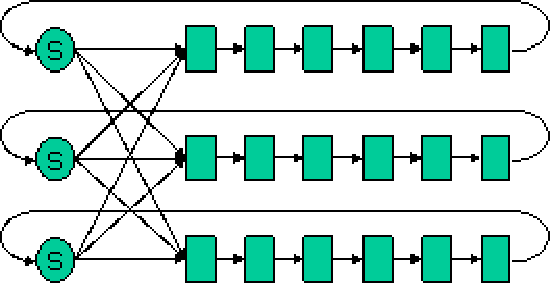
\includegraphics{figures/cqn-model}
    \caption{The Closed Queueing Network (CQN) model}
    \label{fig:cqn-model}
  \end{center}
\end{figure}

To run the model in parallel, we assign tandems to different LPs
(Figure \ref{fig:cqn-partitioning}). Lookahead is provided
by delays on the marked links.

\begin{figure}[htbp]
  \begin{center}
    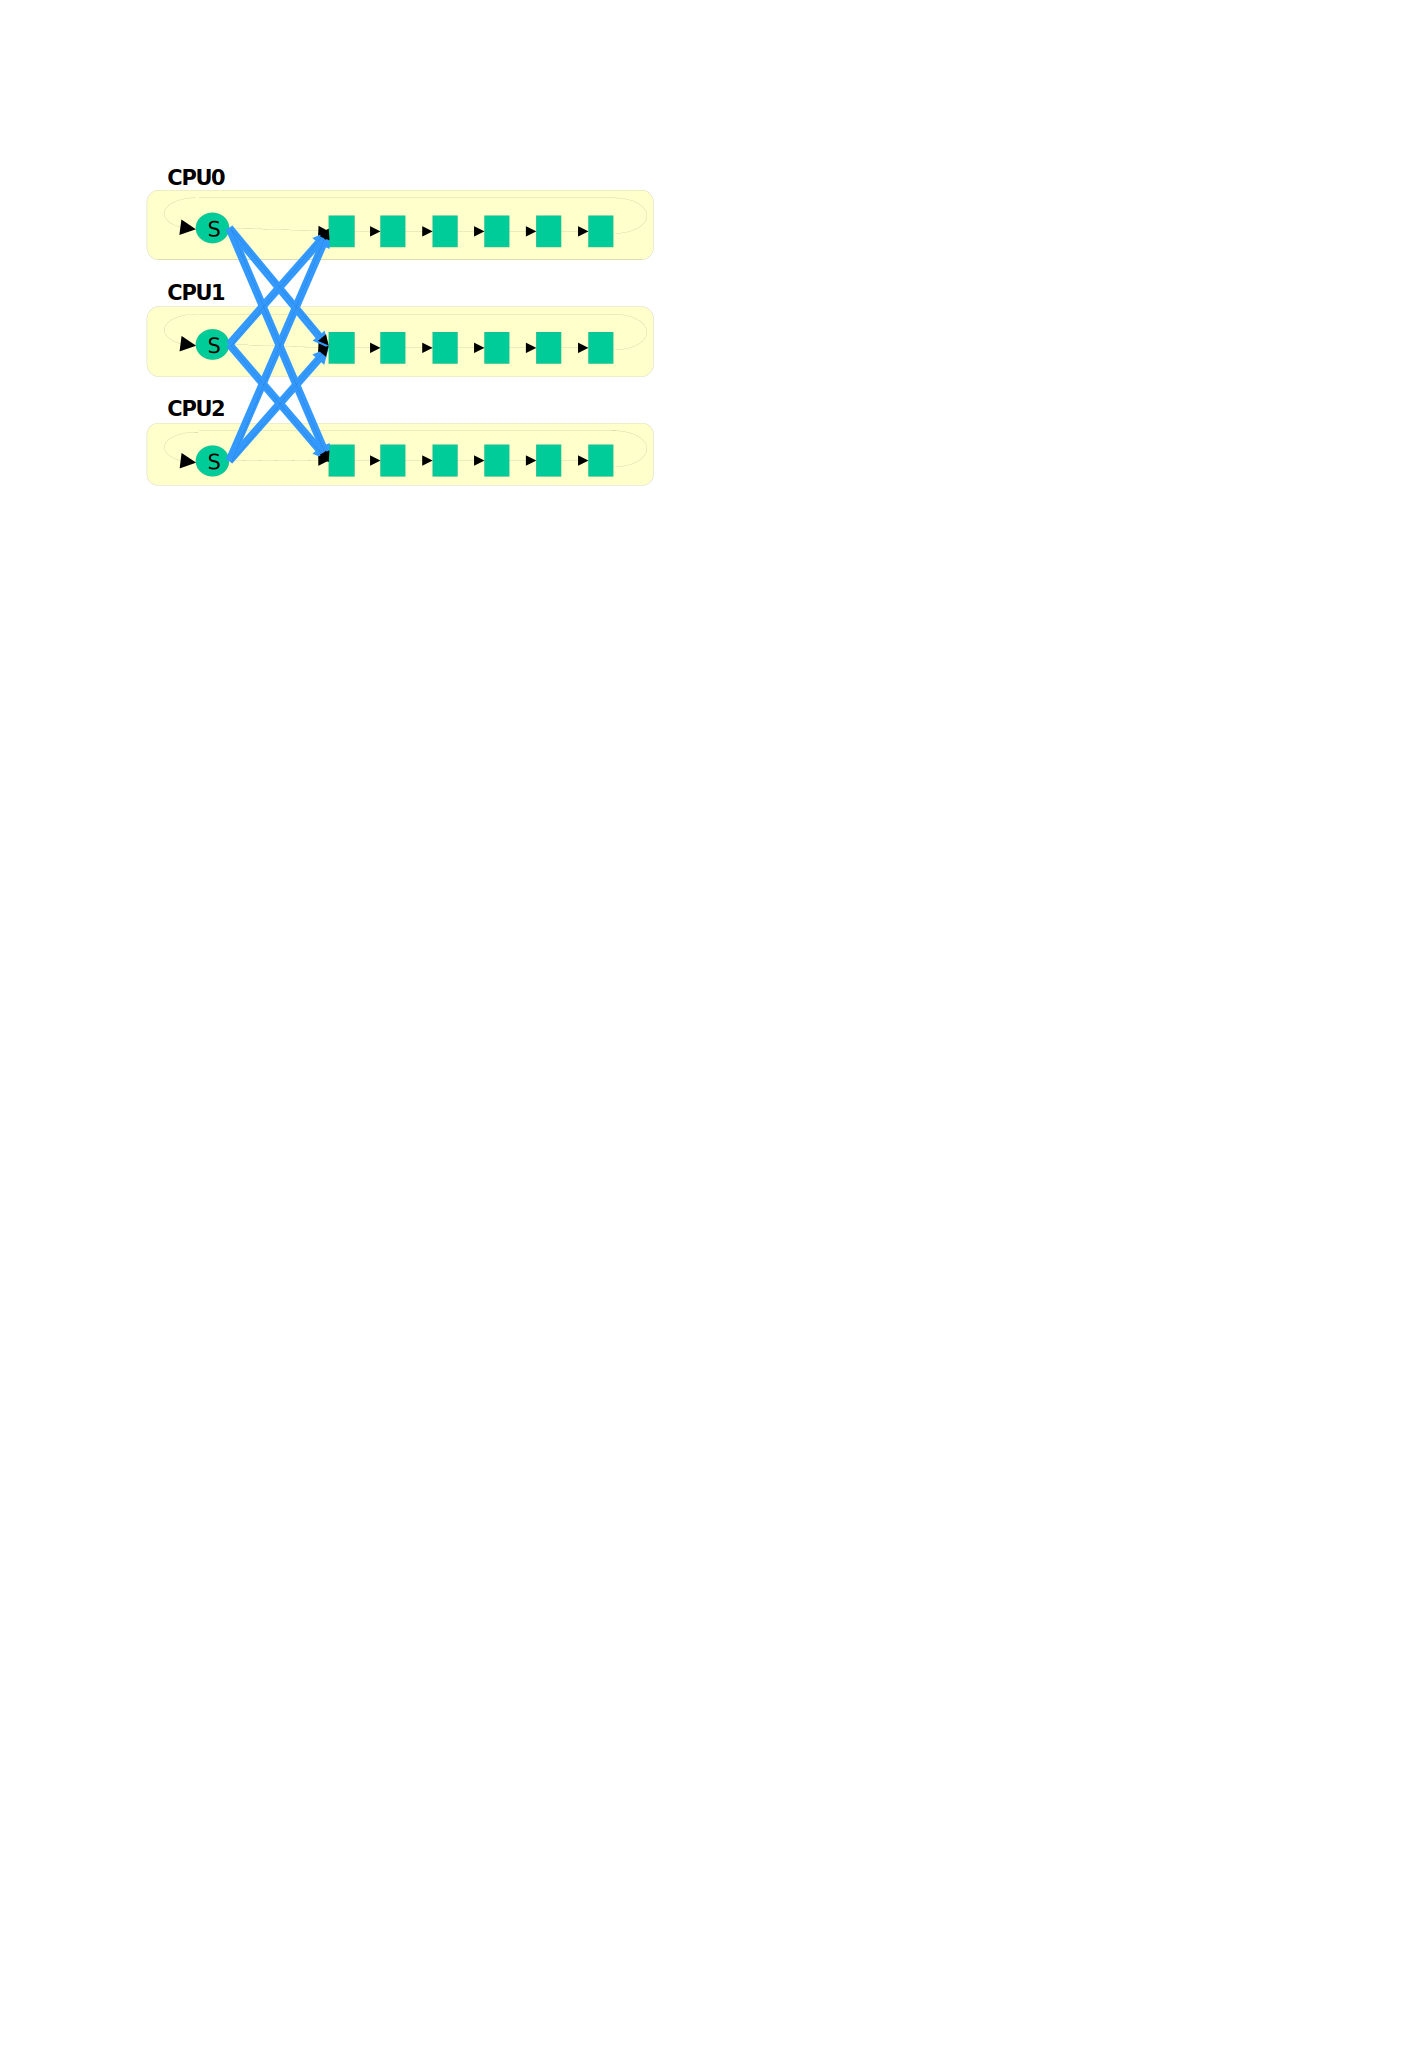
\includegraphics{figures/cqn-partitioning}
    \caption{Partitioning the CQN model}
    \label{fig:cqn-partitioning}
  \end{center}
\end{figure}

To run the CQN model in parallel, we have to configure it for parallel
execution. In {\opp}, the configuration is in a text file called
\texttt{omnetpp.ini}. For configuration, first we have to specify
partitioning, that is, assign modules to processors. This is done
with the following lines:

\begin{verbatim}
[Partitioning]
*.tandemQueue[0].partition-id = 0
*.tandemQueue[1].partition-id = 1
*.tandemQueue[2].partition-id = 2
\end{verbatim}

The numbers after the equal sign identify the LP.

Then we have to select the communication library and the parallel
simulation algorithm, and enable parallel simulation:

\begin{verbatim}
[General]
parallel-simulation=true
parsim-communications-class = "cMPICommunications"
parsim-synchronization-class = "cNullMessageProtocol"
\end{verbatim}

When the parallel simulation is run, LPs are represented
by multiple running instances of the same program.
When using LAM-MPI \cite{lammpi}, the mpirun program (part of LAM-MPI)
is used to launch the program on the desired processors.
When named pipes or file communications is selected, the opp\_prun
{\opp} utility can be used to start the processes.
Alternatively, one can run the processes by hand (the -p flag
tells {\opp} the index of the given LP and the total number of LPs):

\begin{verbatim}
./cqn -p0,3 &
./cqn -p1,3 &
./cqn -p2,3 &
\end{verbatim}

For PDES, one will usually want to select the command-line user interface,
and redirect the output to files. ({\opp} provides the necessary
configuration options.)

The graphical user interface of {\opp} can also be used
(as evidenced by Figure \ref{fig:parsim-screenshot}),
independent of the selected communication mechanism.
The GUI interface can be useful for educational or demonstation purposes.
{\opp} displays debugging output about the Null Message Algorithm,
EITs and EOTs can be inspected, etc.


%Note that results might not be exactly the same, because with PDES,
%random number generators are no longer shared between modules in LPs...



\begin{figure}[htbp]
  \begin{center}
    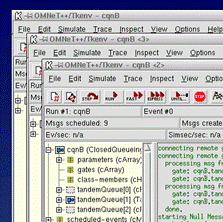
\includegraphics{figures/parsim-screenshot}
    \caption{Screenshot of CQN running in three LPs}
    \label{fig:parsim-screenshot}
  \end{center}
\end{figure}



\subsection{Placeholder modules, proxy gates}

When setting up a model partitioned to several LPs,
{\opp} uses placeholder modules and proxy gates.
In the local LP, placeholders represent sibling submodules
that are instantiated on other LPs.
With placeholder modules, every module has all of its siblings
present in the local LP -- either as placeholder or as the ``real thing''.
Proxy gates take care of forwarding messages to the LP where
the module is instantiated (see Figure \ref{fig:plach}).

The main advantage of using placeholders is that algorithms such as
topology discovery embedded in the model can be used with PDES unmodified.
Also, modules can use direct message sending to any sibling module,
including placeholders. This is so because the destination of direct message
sending is an input gate of the destination module -- if the destination
module is a placeholder, the input gate will be a proxy gate which
transparently forwards the messages to the LP where the ``real'' module
was instantiated. A limitation is that the destination of direct message
sending cannot be a \textit{submodule} of a sibling (which is
probably a bad practice anyway, as it violates encapsulation),
simply because placeholders are empty and so its submodules are
not present in the local LP.

Instantiation of compound modules is slightly more complicated.
Since submodules can be on different LPs, the compound module may
not be ``fully present'' on any given LP, and it may forced to be
present on several LPs (wherever it has submodules instantiated).
Thus, compound modules are instantiated wherever they have
at least one submodule instantiated, and are represented by placeholders
everywhere else (Figure \ref{fig:inst}).


\begin{figure}[htbp]
  \begin{center}
    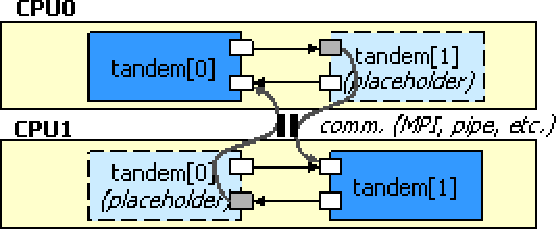
\includegraphics{figures/placeholders}
    \caption{Placeholder modules and proxy gates}
    \label{fig:plach}
  \end{center}
\end{figure}

\begin{figure}[htbp]
  \begin{center}
    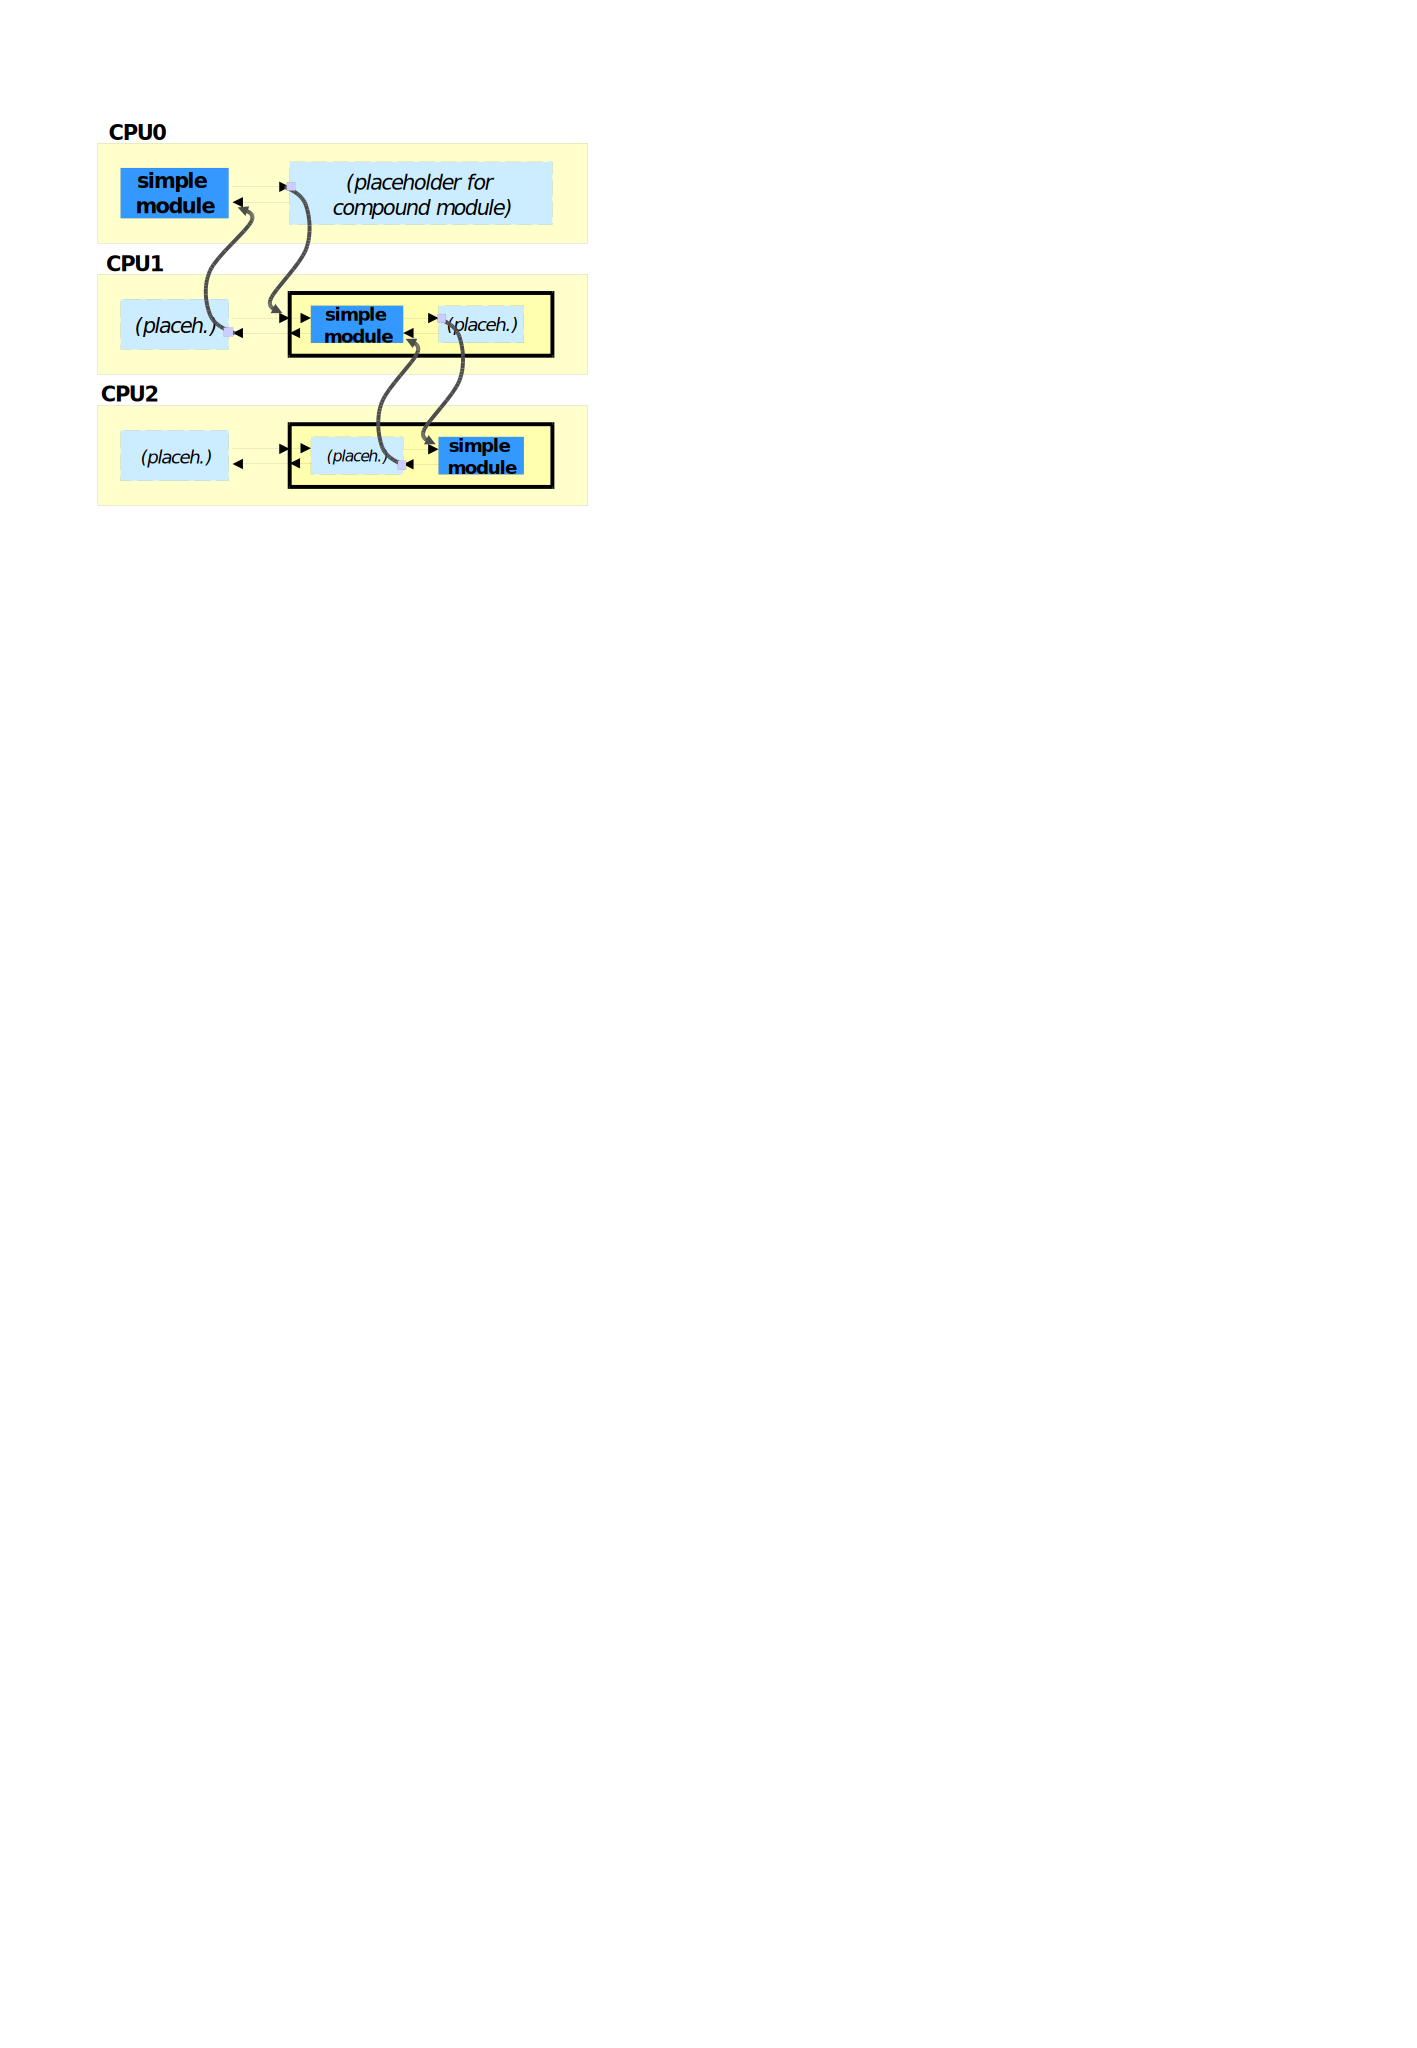
\includegraphics{figures/placeholders2}
    \caption{Instantiating compound modules}
    \label{fig:inst}
  \end{center}
\end{figure}


\subsection{Design of PDES Support in {\opp}}

Design of PDES support in {\opp} follows a layered approach,
with a modular and extensible architecture. The overall
architecture is depicted in Figure \ref{fig:parsim-arch}.

\begin{figure}[htbp]
  \begin{center}
    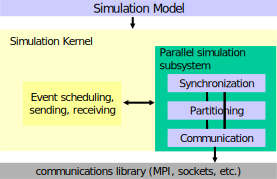
\includegraphics{figures/parsim-arch}
    \caption{Architecture of {\opp} PDES implementation}
    \label{fig:parsim-arch}
  \end{center}
\end{figure}

The parallel simulation subsytem is an optional component
itself, which can be removed from the simulation kernel
if not needed. It consists of three layers, from the bottom up:
communication layer, partitioning layer and synchronization layer.

The purpose of the \textit{Communication layer} is to
provide elementary messaging services between partitions for
upper layer. The services include send, blocking receive,
nonblocking receive and broadcast. The send/receive operations
work with \textit{buffers}, which encapsulate packing and unpacking
operations for primitive C++ types. The message class and
other classes in the simulation library can pack and unpack
themselves into such buffers. The Communications layer API
is defined in the \texttt{cFileCommunications} interface
(abstract class); concrete implementations like the MPI
one (\texttt{cMPICommunications}) subclass from this,
and encapsulate MPI send/receive calls. The matching buffer
class \texttt{cMPICommBuffer} encapsulates MPI pack/unpack
operations.

The \textit{Partitioning layer} is responsible for instantiating
modules on different LPs according to the partitioning specified
in the configuration, for configuring proxy gates.
During the simulation, this layer also ensures that cross-partition
simulation messages reach their destinations. It intercepts messages
that arrive at proxy gates and transmits them to the destination LP
using the services of the communication layer. The receiving LP
unpacks the message and injects it at the gate pointed to be the
proxy gate. The implementation basically encapsulates the
\texttt{cParsimSegment}, \texttt{cPlaceHolderModule},
\texttt{cProxyGate} classes.

The \textit{Synchronization layer} encapsulates the parallel
simulation algorithm. Parallel simulation algorithms are also represented
by classes, subclassed from the \texttt{cParsimSynchronizer} abstract class.
The parallel simulation algorithm is invoked on the following hooks:
event scheduling, processing model messages outgoing from the LP,
and messages (model messages or internal messages) arriving
from other LPs. The first hook, event scheduling is a function
invoked by the simulation kernel to determine the next simulation
event; it also has full access to the future event list (FEL) and
can add/remove events for its own use.
Conservative parallel simulation algorithms will use this hook
to block the simulation if the next event is unsafe, e.g. the
null message algorithm implementation (\texttt{cNullMessageProtocol})
blocks the simulation if an EIT has been reached until a null message
arrives (see \cite{bagrodia00} for terminology); also it uses
this hook to periodically send null messages. The second hook
is invoked when a model message is sent to another LP;
the null message algorithm uses this hook to piggyback null
messages on outgoing model messages. The third hook is invoked
when any message arrives from other LPs, and it allows the
parallel simulation algorithm to process its own internal messages
from other partitions; the null message algorithm processes
incoming null messages here.

The null message protocol implementation itself is modular,
it employs a separate, configurable lookahead discovery object.
Currently only link delay based lookahead discovery has been
implemented, but it is possible to implement more sophisticated
ones.

The Ideal Simulation Protocol (ISP; see \cite{bagrodia00})
implementation consists in fact of two parallel simulation
protocol implementations:
the first one is based on the null message algorithm and
additionally records the external events (events received
from other LPs) to a trace file; the second one executes
the simulation using the trace file to find out which
events are safe and which are not.

Note that although we implemented a conservative protocol,
the provided API itself would allow implementing optimistic
protocols, too. The parallel simulation algorithm has
access to the executing simulation model, so it could perform
saving/restoring model state if model objects support this
  \footnote{Unfortunately, support for state saving/restoration
  needs to be individually and manually added to each class
  in the simulation, including user-programmed simple modules.}.

We also expect that because of the modularity, extensibility and
clean internal architecture of the parallel simulation subsystem,
the {\opp} framework has the potential to become a preferred platform
for PDES research.


%%% Local Variables:
%%% mode: latex
%%% TeX-master: "usman"
%%% End:
